\section{Methods}
\label{methods:general}

To provide better visual objects separation, we focus on adding visual highlighting information to the original picture
changing original brightness of the objects. Initially (see \autoref{methods:processing}), we convert the original image to grayscale, then we use the saliency model to obtain saliency map information. After that, we run an instance segmentation model on the same original image to get instance segmentation masks of the predefined allowed list of classes). Given the masks, we construct a graph on a base of these masks where objects are vertices, and each edge corresponds to two objects being adjacent to each other. After creating the graph, we apply the graph coloring strategy to assign brightness to these objects and recolor them to separate the objects better (in the \autoref{methods:recoloring}). Given all these layers (saliency map, grayscale image, and colored segmentation results) in \autoref{methods:combining} we combine them together to produce the final result to be provided to the user. Finally, in {\autoref{methods:survey}} to evaluate the results, we processed our images with the pulse2percept (p2p) model and conducted a user study in order to measure the improvement.

\begin{figure*}
    \begin{subfigure}[t]{0.16\linewidth}
        \centering
        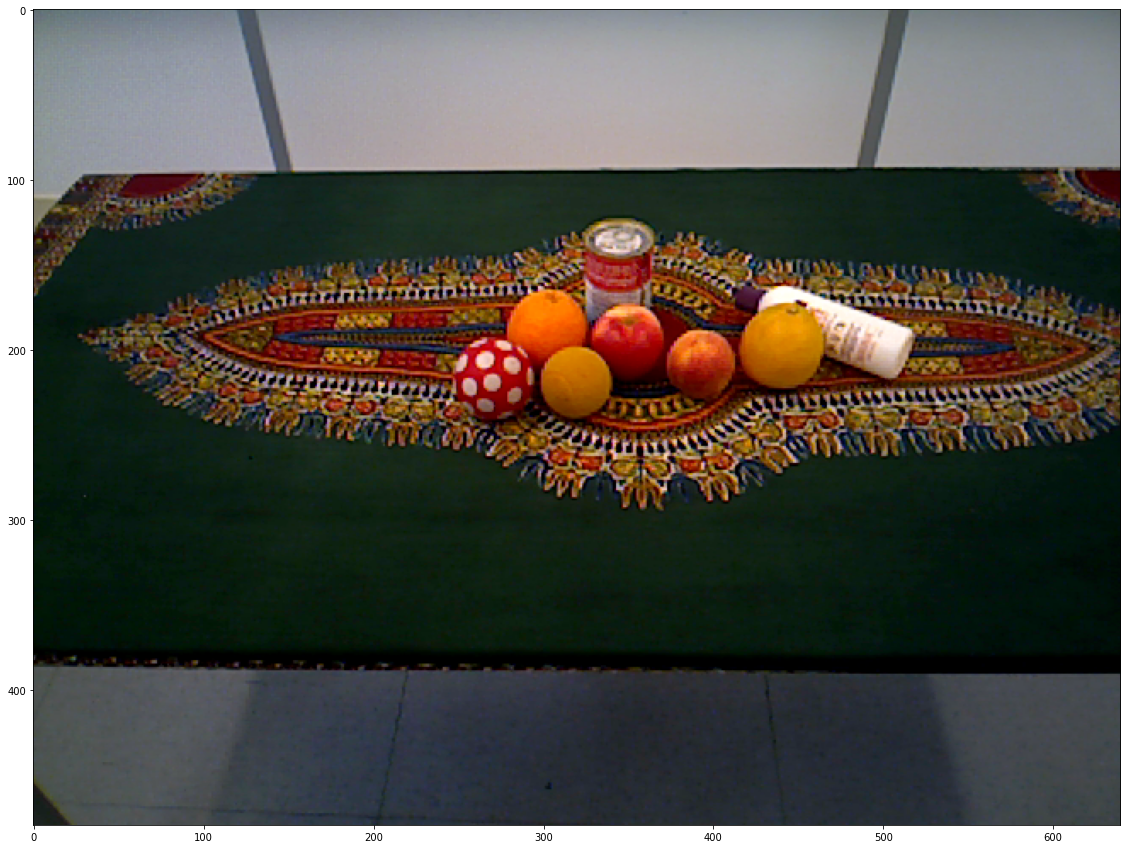
\includegraphics[width=\textwidth]{figures/methods1.png}
        \caption{Initial RGB}
        \label{methods:pic1}
    \end{subfigure}
    \hfill
    \begin{subfigure}[t]{0.16\linewidth}
        \centering
        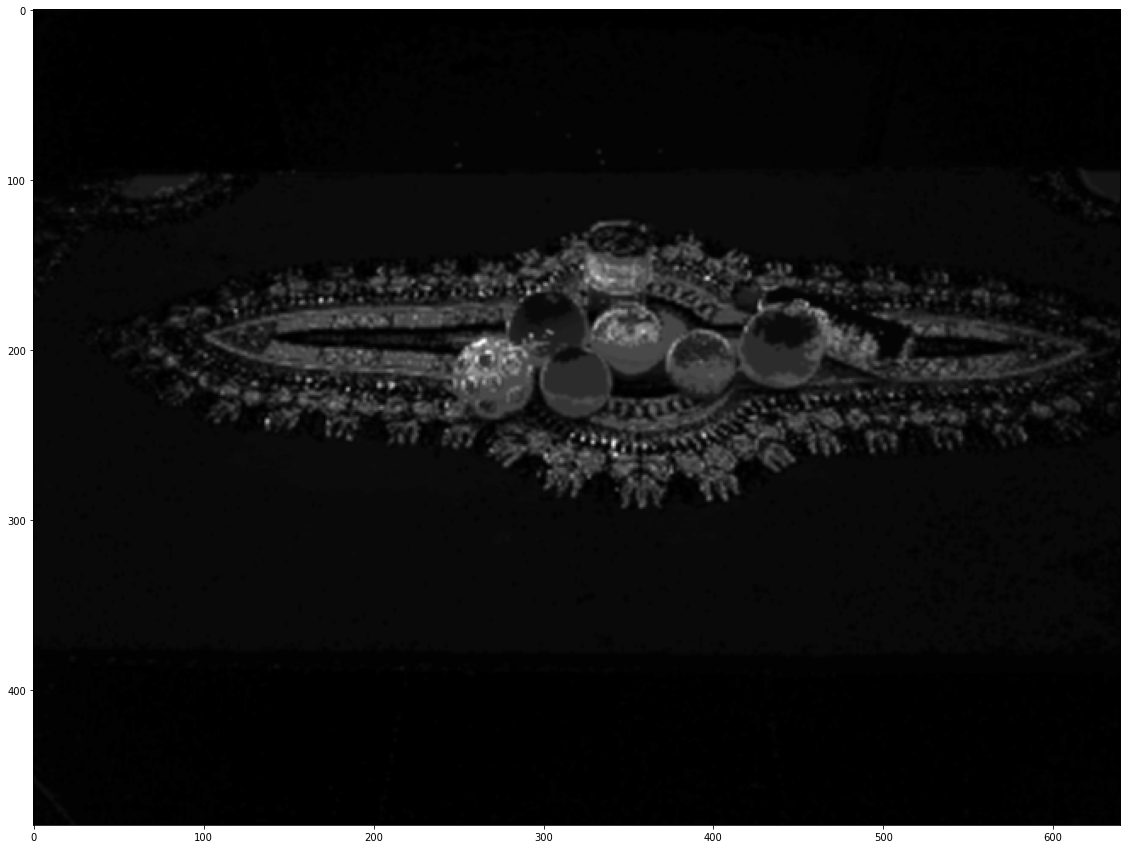
\includegraphics[width=\textwidth]{figures/methods2.png}
        \caption{Saliency map}
        \label{methods:pic2}
    \end{subfigure}
    \hfill
    \begin{subfigure}[t]{0.16\linewidth}
        \centering
        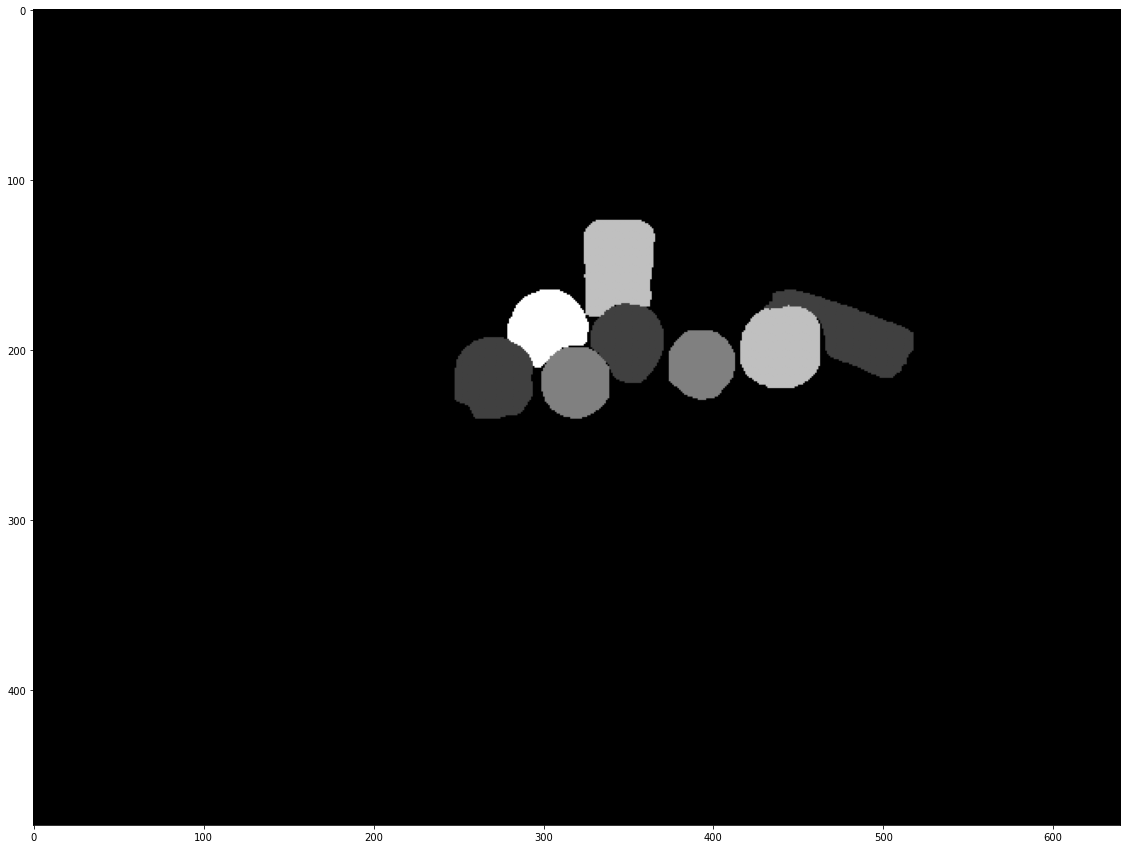
\includegraphics[width=\textwidth]{figures/methods3.png}
        \caption{Segmentation before recoloring}
        \label{methods:pic3}
    \end{subfigure}
    \hfill
    \begin{subfigure}[t]{0.16\linewidth}
        \centering
        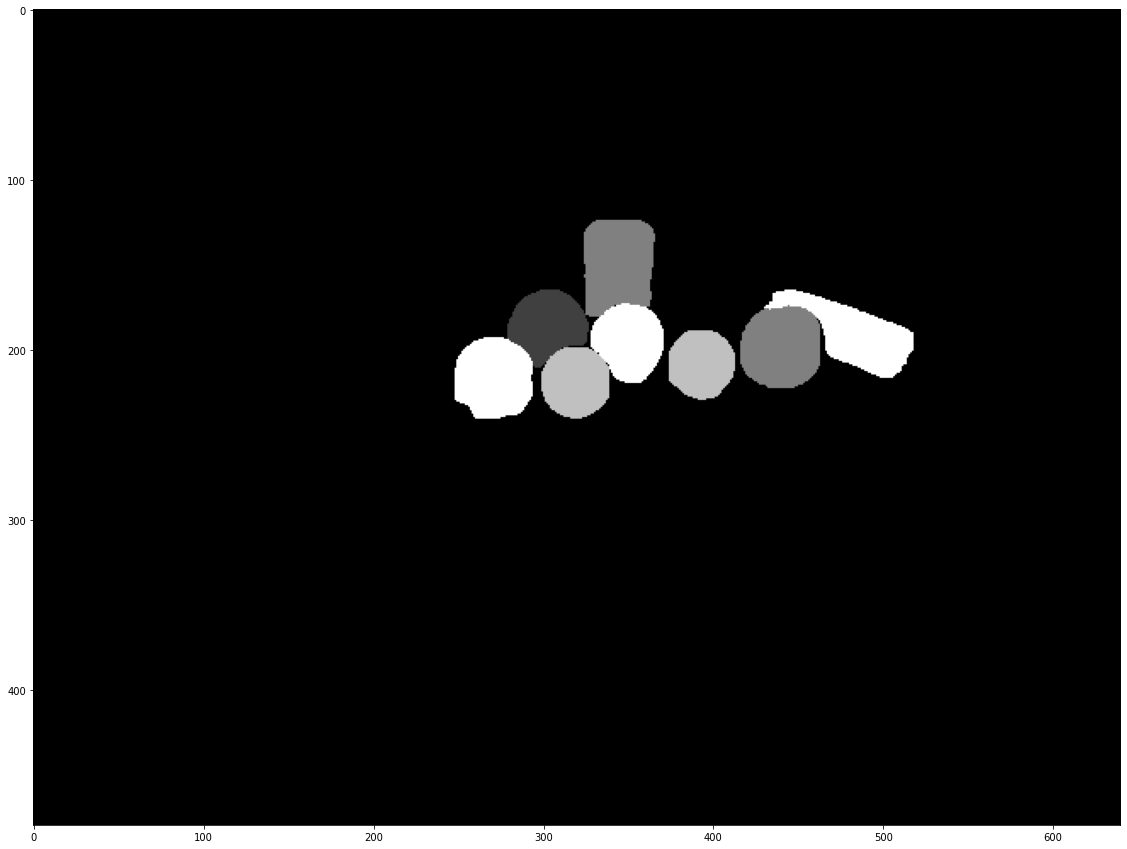
\includegraphics[width=\textwidth]{figures/methods4.png}
        \caption{Segmentation after recoloring}
        \label{methods:pic4}
    \end{subfigure}
    \hfill
    \begin{subfigure}[t]{0.16\linewidth}
        \centering
        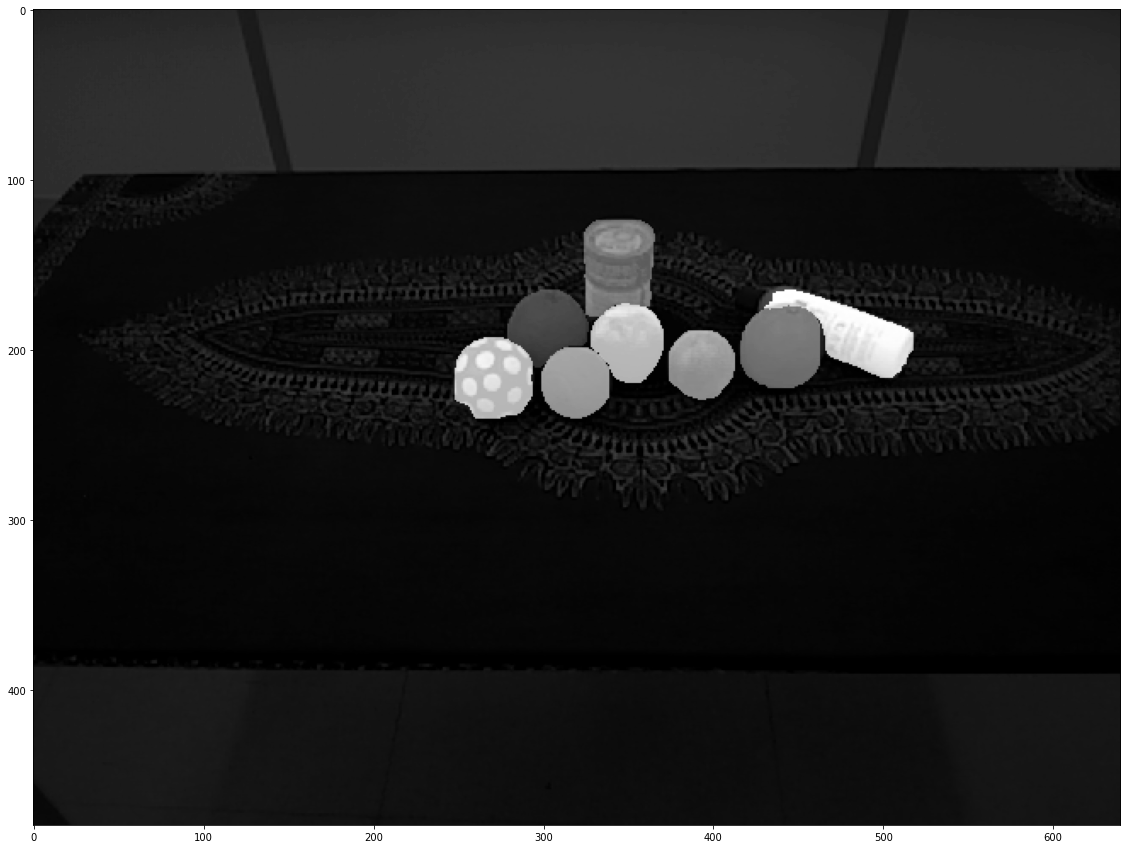
\includegraphics[width=\textwidth]{figures/methods5.png}
        \caption{Our result}
        \label{methods:pic5}
    \end{subfigure}
    \newline
    \begin{subfigure}[t]{0.16\linewidth}
        \centering
        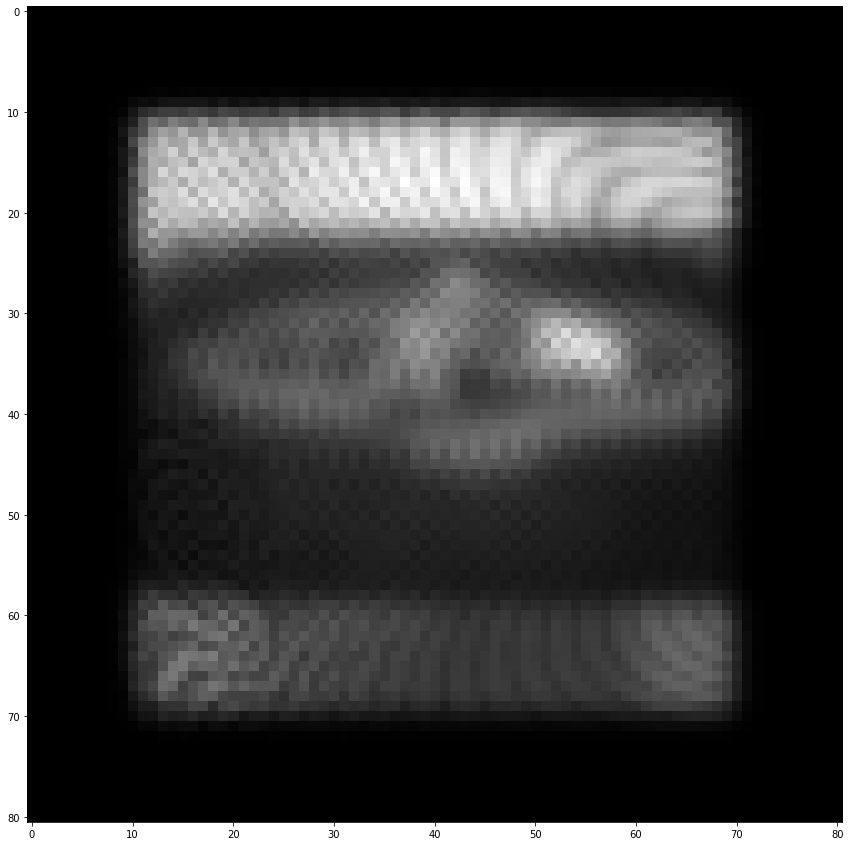
\includegraphics[width=\textwidth]{figures/methods6.png}
        \caption{p2p: initial RGB}
        \label{methods:pic6}
    \end{subfigure}
    \hfill
    \begin{subfigure}[t]{0.16\linewidth}
        \centering
        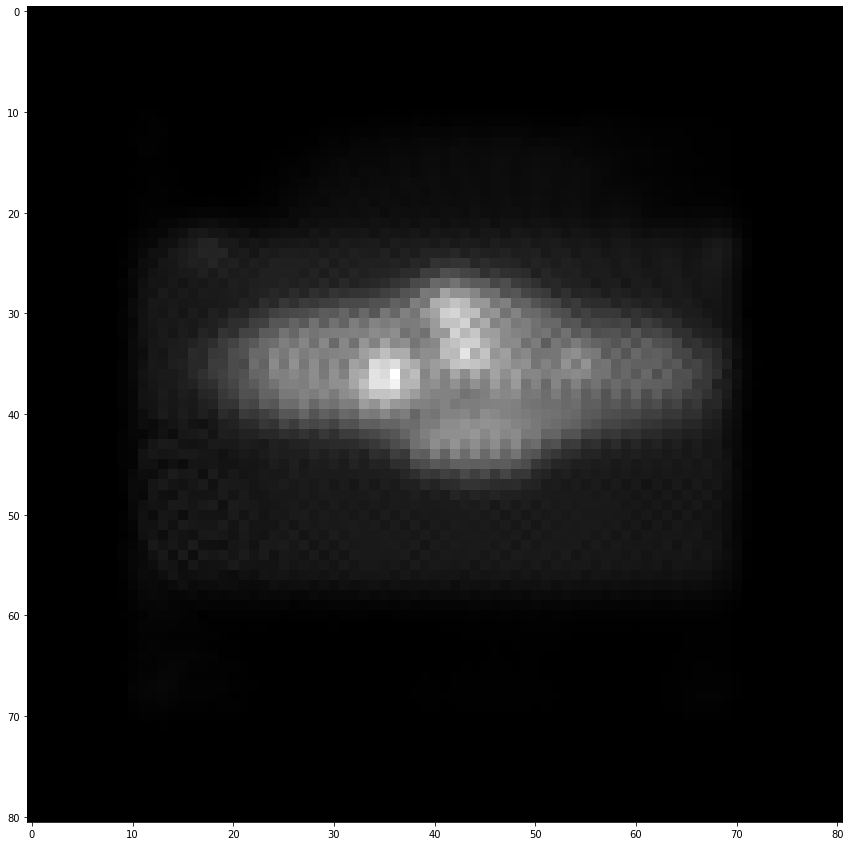
\includegraphics[width=\textwidth]{figures/methods7.png}
        \caption{p2p: saliency map}
        \label{methods:pic7}
    \end{subfigure}
    \hfill
    \begin{subfigure}[t]{0.16\linewidth}
        \centering
        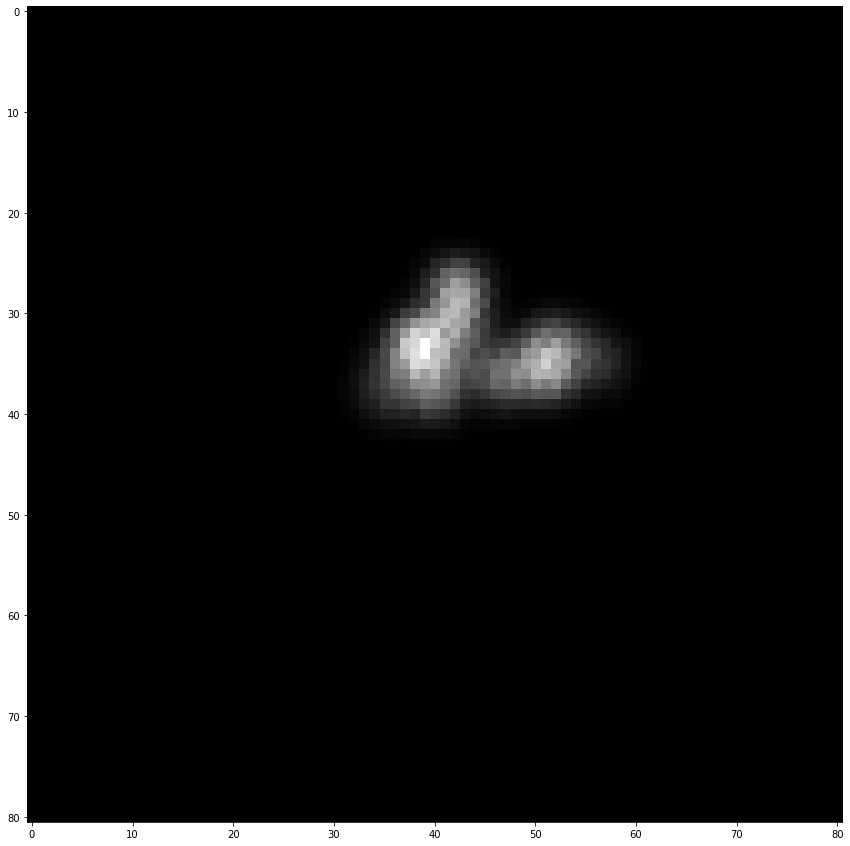
\includegraphics[width=\textwidth]{figures/methods8.png}
        \caption{p2p: segmentation before recoloring}
        \label{methods:pic8}
    \end{subfigure}
    \hfill
    \begin{subfigure}[t]{0.16\linewidth}
        \centering
        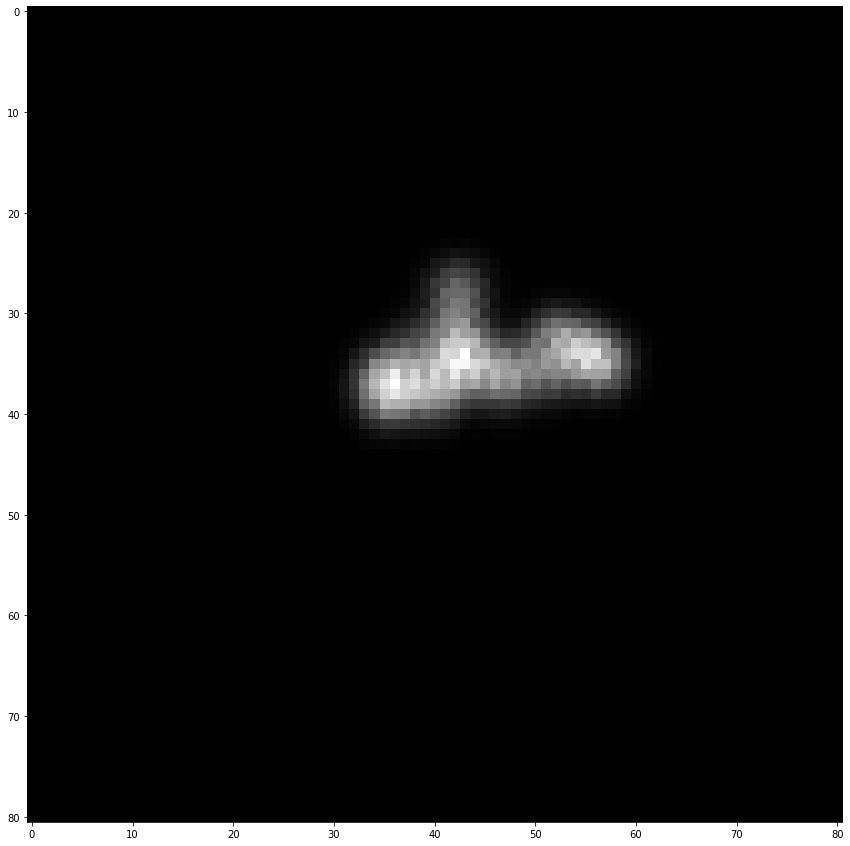
\includegraphics[width=\textwidth]{figures/methods9.png}
        \caption{p2p: segmentation after recoloring}
        \label{methods:pic9}
    \end{subfigure}
    \hfill
    \begin{subfigure}[t]{0.16\linewidth}
        \centering
        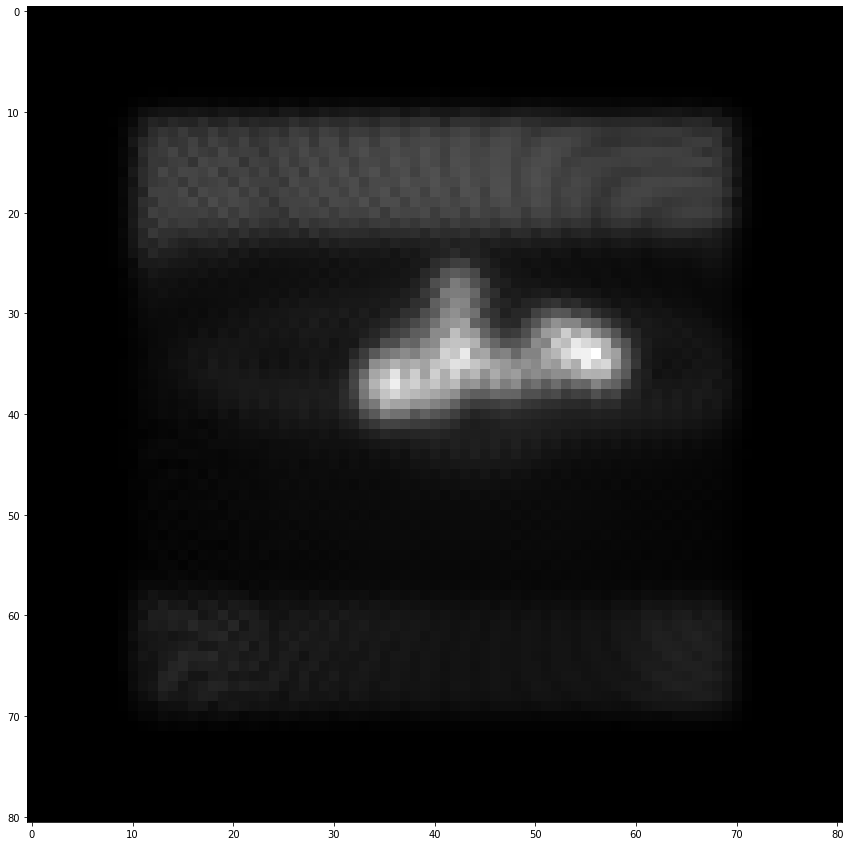
\includegraphics[width=\textwidth]{figures/methods10.png}
        \caption{p2p: our result}
        \label{methods:pic10}
    \end{subfigure}
    \caption{Stages of processing the picture and corresponding visualizations via pulse2percept.}
    \label{methods:picture}
    \Description{Initially, the image is converted to grayscale, then the saliency map and segmentation map are obtained. After that, all these maps and grayscale images are combined in the resulting image. Finally, visualization via pulse2percept is added to show improvements to bionic vision implant users.}
\end{figure*}


\subsection{Dataset}
\label{methods:dataset}

We chose Object Clutter Indoor Dataset \cite{ociddataset} to use as visual stimuli for our research.
This dataset provides 96 different cluttered indoor scenes with different objects that you can find in the room. 
Each scene is located on either floor or the table and represents a typical scenario where the bionic implant user needs to find an object in a pile of similar objects or near some background. We chose a subset of pictures from the dataset to reduce calculations but tried to keep different backgrounds to make the research more representative.
For each picture from the dataset, there exist RGB picture, point cloud, depth map, and label information, but we kept only RGB to represent the most popular RGB video cameras suited for implants. Initial RGB image and corresponding p2p visualization are provided on \autoref{methods:pic1} and \autoref{methods:pic6}.

\subsection{Processing the image}
\label{methods:processing}

As we design our solution for daily indoor scenarios, we need to keep original picture information and provide it to the user.
Considering the current restrictions of bionic vision implants, we convert the image to grayscale using standard conversion weights. In addition to it, we extract saliency map information (see \autoref{methods:pic2} and \autoref{methods:pic7} for saliency map and p2p perception of saliency map correspondingly) from the original color image using the DeepGaze II model \cite{kmmerer2016deepgaze}. Saliency models predict how people look in images and provide valuable feedback on what places to highlight, as this would be interesting to pay attention to. Given that the original background would be dimmer than before, we believe it is important to highlight important places and structures besides the objects as this information can be critical. 

In parallel to saliency reconstruction, we invoke a segmentation algorithm on the original color image. We use detectron2 model \cite{wu2019detectron2} with pretrained weights on LVIS dataset \cite{gupta2019lvis} named 'X101-FPN' in the detectron2 Model Zoo. The LVIS dataset is a dataset for large vocabulary instance segmentation that incorporates more than 1200 categories of objects, including typical indoor objects like fruits, pens, and others. This dataset is, to our knowledge, the best-suited dataset for indoor instance object segmentation with pre-trained models available in detectron2 Model Zoo. After segmentation, we filter the results and keep only masks of classes from the predefined allowed list of classes where we enlisted the most popular indoor objects categories available in the LVIS dataset. This list intentionally does not contain several classes (like table, carpet, and others) as these objects are usually not the target to be found by bionic vision users. In addition to filtering the classes, we also remove objects whose size is less than certain hyperparameters. Besides that, we also look for pair of objects which intersect heavily and remove one of them. We calculate Intersection-Over-Union (IoU) metrics for that.

After segmentation masks are obtained, we construct a graph from these masks. As segmentation only provides us a list of objects to highlight, we need to properly assign them different brightness to make them easily visually separable from each other. To achieve this, we create an adjacency graph of these objects where each node corresponds to an object, and if two objects are close to each other on the image (so the distance between their closest points is less than the corresponding hyperparameter), then the edge between these objects is created. This graph later is subject to the graph coloring algorithm. This algorithm tries to assign different colors to adjacent nodes, which greatly fits our strategy of highlighting the adjacent objects differently to make them different. We use standard greedy algorithm \cite{kubale2004graph} with largest\_first strategy. After coloring is finished, the adjacent objects are assigned different color classes, and the whole graph (and therefore the whole image) uses the least possible amount of colors. As for the grayscale image only changes in brightness are available, reducing the overall amount of classes increases the brightness difference between the classes and makes objects of different color classes more distinguishable. Results of coloring and corresponding p2p perception are provided on \autoref{methods:pic3} and \autoref{methods:pic8}.

\subsection{Recoloring}
\label{methods:recoloring}

The main disadvantage of the graph coloring algorithm is a lack of ordering in coloring. For example, given object A with color class 1, for the coloring algorithm there is no difference in assigning classes 2 or 3 to the adjacent objects. However, as we want adjacent objects to be not only different but most possibly different, we want to assign the most different brightness values to adjacent objects. To achieve this, we use recoloring strategy on top of the resulting colored graph.

The primary purpose of recoloring strategy is to make static mapping between current color classes assigned to each node to new color classes where the difference between adjacent objects increases. This mapping is global for the whole graph, so if the strategy decides to change color class 1 to color class 5, this change would be applied to all color class 1 objects (so they become of color class 5), and no more color classes would be mapped to color class 5. As we plan to directly transform color classes to corresponding brightness levels, we value the situation where objects of color classes 1 and 5 are adjacent greater than where the same objects are of color classes 1 and 2. To reassign the labels, we created several different recoloring strategies.

The currently used recoloring strategy is based on top of the breadth-first search algorithm. It starts with a random node, assigns the biggest class to this node, and takes all neighbors whose classes are not reassigned yet. Next, all these neighbors classes are reassigned, so they differ the most from the current node and each other, and then the algorithm deletes assigned color classes from the list of available color classes and recursively starts from these nodes, and works until all classes are remapped.

We noticed that this algorithm, on average, produces better coloring results than the default coloring greedy strategy and other recoloring algorithms, but this statement is yet to be proved via user survey in future work.

After recoloring the graph, we provide these labels to the objects and transfer them to the single two-dimensional layer to be used later in combination with other layers. Results of recoloring and corresponding p2p perception are provided on \autoref{methods:pic4} and \autoref{methods:pic9}.

\subsection{Combining the results}
\label{methods:combining}

The resulting segmentation map is being rescaled to the $[0.255]$ range to be treated as a valid greyscale image. This map alone theoretically could be passed to bionic implant users, but it would pose a risk of hiding the objects not being recognized but still crucial for the user.

To provide background information for the segmented objects, we would like to add more information on the recolored segmentation maps. Therefore, we tried several mixing methods and concluded that combining grayscale maps and recolored segmentation maps would bring the best result.

We first tried to combine the saliency map and the recolored segmentation map by modifying the method given in the previous paper \cite{han2021deep}, as the saliency maps can include the region of interest in the background. We first thresholded the saliency map to only retain 30\% of the most salient region and then added them to the place where nothing is segmented in the recolored segmentation map. However, the combined map only adds small undistinguishable artifacts on the recolored segmentation map. When we transform it into simulated prosthetic images, it does not introduce significant changes to the simulated prosthetic images transformed from the recolored segmentation map.

We then tried to combine the grayscale map and the recolored segmentation map. The grayscale map would be x\% percent of the combined image, and the recolored segmentation map would be (100-x\%) percent of the image. We tried many x values and suggested that 30 would be the best value to include information in the grayscale map differentiated from the recolored segmentations.
To make the grayscale map much clearer in low percentage in the combined map, we tried thresholding the grayscale map into binary. However, thresholding introduce significant changes in the shape of the background objects (like tables) that make the background hard to understand both the combined map and in simulated prosthetic vision images. We also tried adding contrast to the grayscale map, but the resulting prosthetic images are similar to the ones without adding contrast.

The final combination and corresponding p2p perception are provided on \autoref{methods:pic5} and \autoref{methods:pic10}. Additional examples of full processing pipeline could be found on \autoref{appendices:processing}.

\subsection{User study}
\label{methods:survey}

To estimate the changes, we considered surveying objects' distinguishability on images as bionic implant users see them. 
The processed images from previous steps were then transformed into simulated prosthetic images using open-source library pulse2percept \cite{Beyeler148015}. The images would be the input stimuli to the pulse2percept simulator. The simulator downscaled the processed images into the electrode array size and assigned each pixel in the processed image to an electrode. The grayscale value of the pixel determines the current on the electrodes. The size of the electrode array in our simulation is 32x32, which is a possible size of an electrode array in current or developing retinal implants, and shows good performance on identifying people and cars in the outdoors scene in the previous paper \cite{han2021deep}.

We used the axon map model in the pulse2percept library. The shape of the phosphene in the model is determined by parameters rho and axlambda, where rho is the exponential decay constant away from the axon and axlambda is the exponential decay constant along the axon. Since the actual phosphene shape varies among patients, we tried several possible pair of rho and axlambda and chose the one (rho = 70, axlambda = 30) that show the difference in coloring.

We created a subset of 15 randomly chosen images and applied our algorithm to produce versions of them with highlighted objects. Then we processed each image with the chosen pulse2percept model to represent a typical perception of these images by a bionic implant user. We then created a publicly available website where we asked people to estimate the number of objects on the given picture. We neither stated whether this picture was original or preprocessed nor described the research idea to the subjects. 